\documentclass{journal}
\usepackage{graphicx}
\usepackage{amsmath}

\title{Software Defined Modem Using Modern Micro-Controllers}
\author{Joshua Jerred}
\date{\today}

\begin{document}
\maketitle

\section{Introduction}

Modern embedded hardware is far more capable than it has been in the past. Newer devices, such as the STM32, have powerful ARM cores matched up with other hardware inside of small single chip MCU packages. With peripherals like ADCs and DACs, along side DMA, audio can be cleanly generated in real time. This can be used to generate modulated data streams, with one common piece of hardware.

\section{Background}

\section{Hardware}
The idea of this project is that a generic microcontroller (MCU) is capable of acting as a software defined modem. Given this, the hardware will be kept simple. A single MCU will be used to act as the software modem. The modem will be connected to an external host/client, this client will control the modem. The modem has a single audio output and audio input, this can connected to various types of physical mediums to transfer the data that is modulated in the audio from one modem to another.

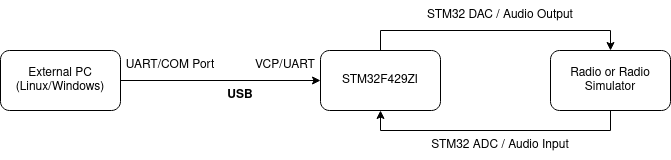
\includegraphics[width=4in]{images/hardware_outline}

\begin{center}
\subsection{MCU Requirements/Considerations}
\end{center}

When looking for the appropriate MCU for this project there were a few requirements and considerations that needed to be taken into account.

\begin{itemize}
  \item[ADC] A single ADC (Analog-to-Digital Converter) is required to sample the input audio. It needs suitable resolution and speed to capture the modulated audio stream.
  \item[DAC] A single DAC (Digital-to-Analog Converter) is required to output modulated audio from the microcontroller.
  \item[DMA] DMA (Direct Memory Access) is required to transfer data to/from the ADC/DAC automatically without CPU intervention. Although this may not be strictly required, it will free up a considerable amount of CPU time.
  \item[Hardware Timers] Accurate hardware timers are required for properly timing the audio waveform generation, and the modulation.
  \item[USB/UART] A USB/UART connection is required to connect an external MCU to a host device so that the host device can send/receive data to/from the modem.
  \item[Cost] There are many devices that are capable of completing the task, but the cost of the device is a major consideration. The device should be as cheap and as generic as possible to allow for easy replication of this project on other hardware.
\end{itemize}


\section{Waveform Generation}
\[
  F_{trigger} = \frac{C_{APB1}}{(PSC+1)*(ARR+1)}
\]
where:
\begin{itemize}
  \item[$C_{APB1}$] is the clock frequency of the APB1 bus
  \item[$PSC$] is the prescaler value
  \item[$ARR$] is the auto-reload value
  \item[$F_{trigger}$] is the frequency of the trigger
\end{itemize}

\[
  F_{output} = \frac{F_{trigger}}{N_{samples}}
\]

\section{Software Implementation}
\begin{itemize}
  \item Sine Wave Generation
  \item 
\end{itemize}

\end{document}